\thispagestyle{fancy}
\begin{center}
	\LARGE{\textbf{Resistores en serie}}
\end{center}
\section{Objetivos}

Al analizar esta experiencia, Ud. estará capacitado para:
\begin{enumerate}
	\item Utiliza el DMM como ohmímetro para la medición de resistores conectados en
	serie.
	\item Medir caídas de tensión en resistores conectados en serie.
\end{enumerate}
\section{Conocimientos previos}
Cuando varios resistores se conectan uno a continuación de otro, la misma corriente
circula por todos ellos. Se dice que los resistores están en serie.
Los resistores conectados en serie pueden ser reemplazados por un único resistor
equivalente (Req), sin que esto afecte en modo alguno el funcionamiento del circuito.
La resistencia equivalente serie es:
\begin{equation*}
	R_{eq} = R_{1} + R_{2} + R_{3}+ . . . + R_{n}
\end{equation*}
\section{Autoevaluación de entrada}
\begin{enumerate}
	\item La resistencia equivalente ($R_{eq}$) de resistores conectados en serie es:\\
	La suma aritmética de las resistencias .
	\item La caída de tensión en una red de resistores conectados en serie es igual a:\\
	La suma de las caídas de tensión de todas las resistencias.	
\end{enumerate}
\section{Equipos}
Los siguientes equipos son necesarios para la realización de la experiencia. 
\begin{enumerate}
	\item Módulo de experiencias
	\item DMM (Multímetro digital)	
\end{enumerate}
\section{Procedimiento}
\begin{enumerate}
	\item Estudie la figura 1.
	\begin{enumerate}
		\item Se observa dos resistencias en serie $R_{5}$ y $R_{6}$
		\item Se presencia de un Ohmímetro
		\item El valor de $ R_{5} = 1.8 k\Omega$
		\item	El valor de $R_{6} = 6.8 k\Omega$
	\end{enumerate}
	\item Determine los valores de $R_{5}, R_{6}, R_{7}, R_{8}, R_{9}$ y $R_{10}$, utilizando el código de colores. Mida las resistencias con el multímetro. Registre en la tabla los valores deducidos del código de colores y los valores medidos.
	\\
	\begin{table}[h]
		\centering
		\begin{tabular}{|c|c|c|}
			\hline
			\textbf{Resistor}&\textbf{Valor nominal ($k\Omega$)}& \textbf{Valor medido ($k\Omega$) } \\
				\hline
			$R_{5}$& 1.8&1.76 \\
			\hline
			$R_{6}$& 6.8&6.62 \\
			\hline
			$R_{7}$& 4.7&4.55 \\
			\hline
			$R_{8}$& 1.5&1.52\\
			\hline
			$R_{9}$&2.7&2.65 \\
			\hline
			$R_{10}$& 0.47&0.46 \\
			\hline
		\end{tabular}
		
	\end{table}
	\item Implemente el circuito de la figura 1.
	\begin{figure}[h]
		\centering
		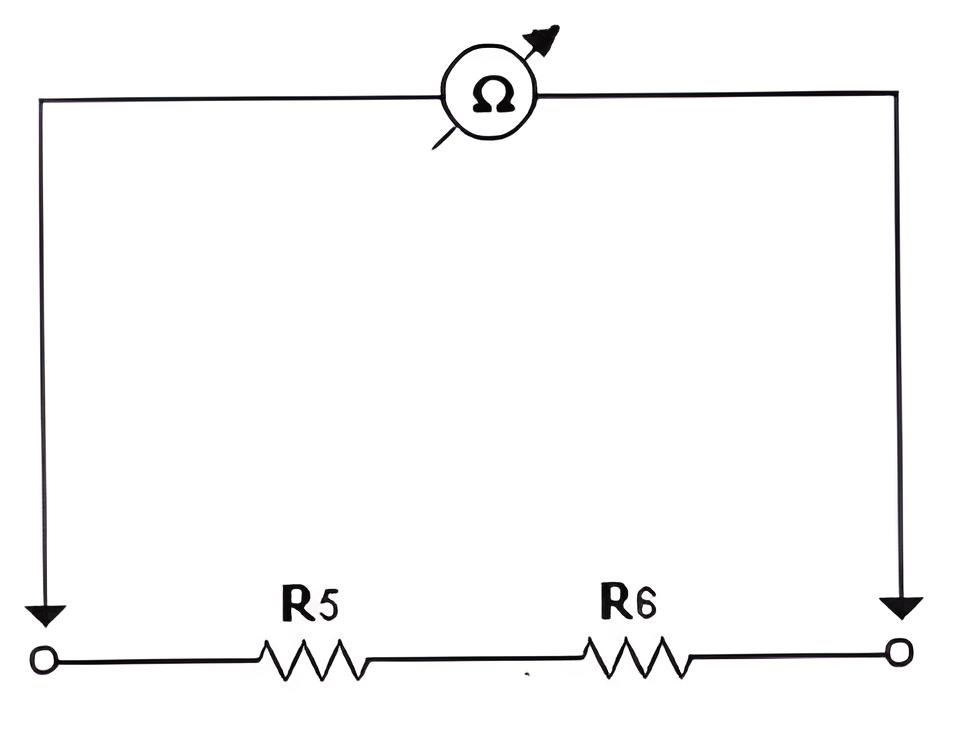
\includegraphics[scale=0.3]{imagenes/1}
	\end{figure}
	\item Mida y registre el valor de la resistencia combinada de R5 y R6.
	Conecte el DMM para medir la resistencia de R5 y R6 como se muestra en la figura 1.\\
	$R_{Medidda} = 8.38 k\Omega $\\
	$R_{Calculada} = 1.8 + 6.8 = 8.6 k\Omega$
	\item Conecte el DMM para medir la resistencia combinada de R7 y R8 como se muestra en la figura 1.\\
	Mida registre el valor de la resistencia combinada de $R_{7}$ y $R_{8}$. 
	$RESISTENCIA SERIE (medida) = 6.01 K\Omega$\\
	$RESISTENCIA SERIE (calculada) = 4.7 + 1.5 = 6.2 k\Omega$
	\item Estudie el siguiente circuito.
	\\
	\\
	\\
	\begin{figure}[h]
		\centering
		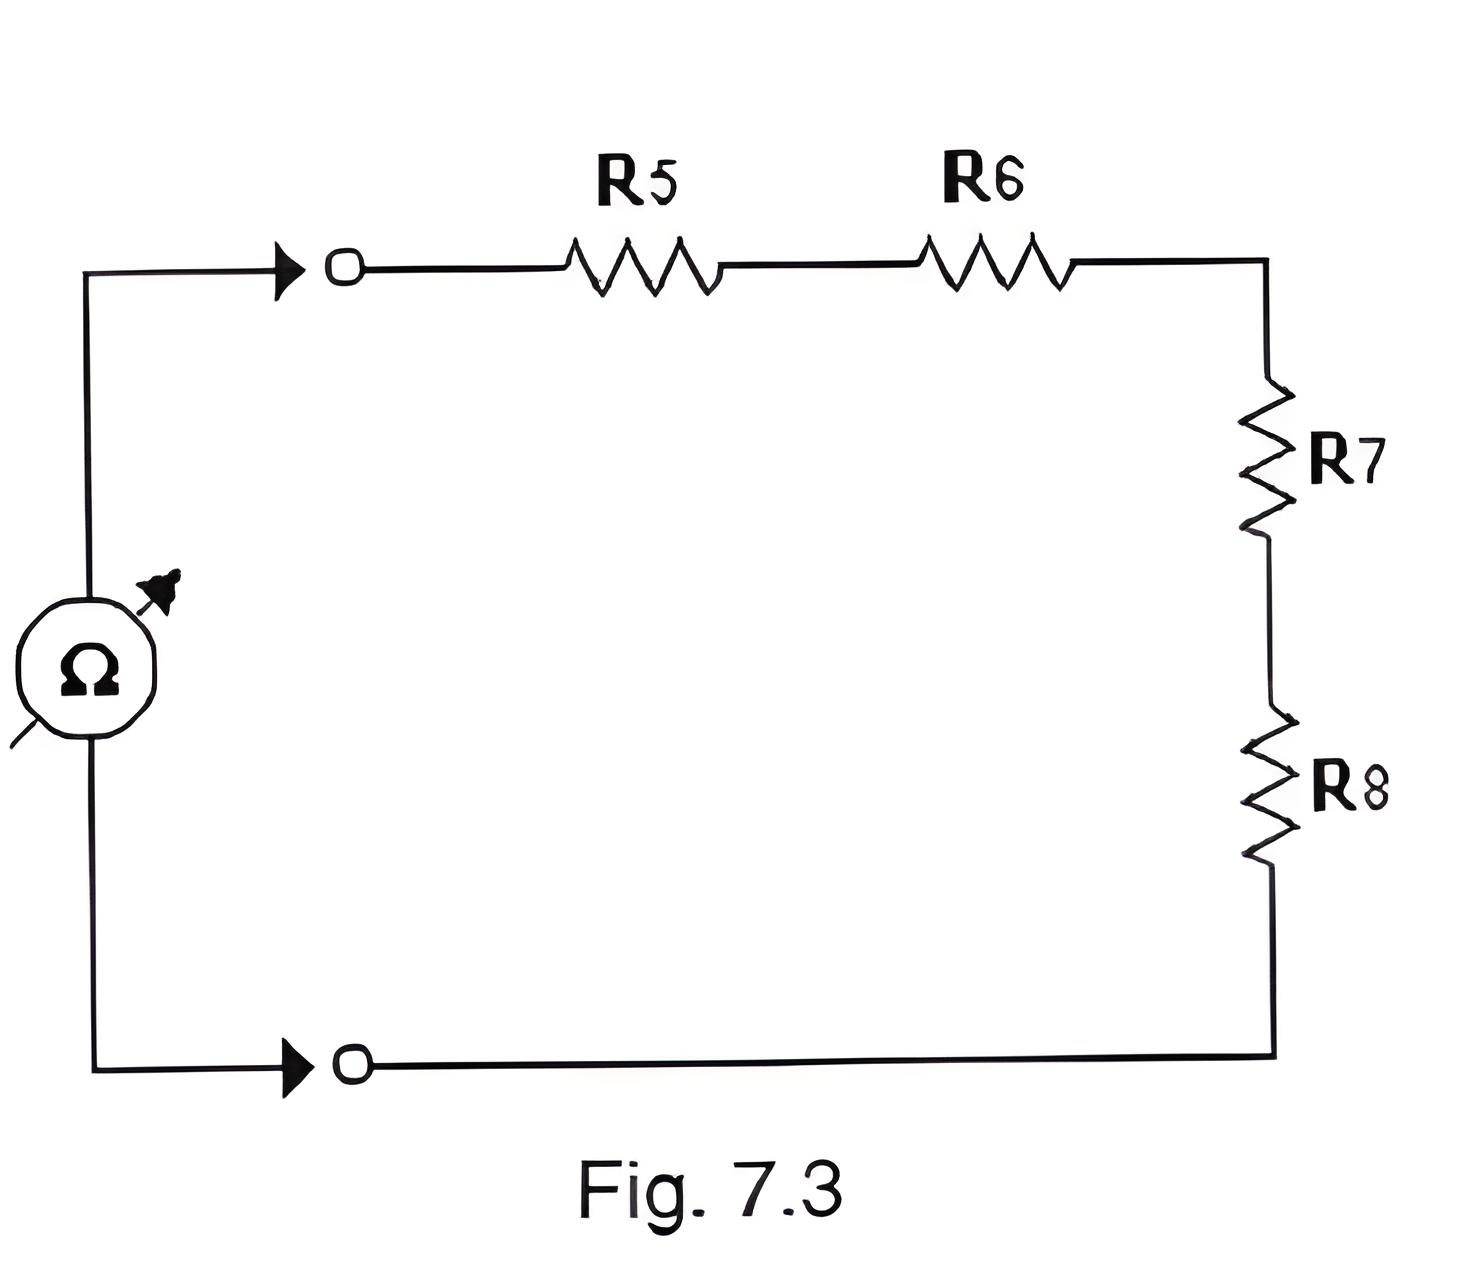
\includegraphics[scale=0.3]{imagenes/2}
	\end{figure}
	\item Conecte las cuatro resistencias del modo mostrado en la figura 3
	Mida y registre el valor de las resistencias combinadas de $R_5, R_{6}, R_{7}$ y $R_{8}$. 
	\\ $R_{Medida}=14.39k\Omega$
	\\ $R_{Calculada}=14.k\Omega$
	\\ \textbf{En esta parte del experimento, el modo de práctica, el circuito sufrirá una serie de cambios.}
	\\ \textbf{Ud. Deberá hablar qué componentes han sido modificados.}
	\item $R_{5}$ ha sido modificada. Mida y registre el valor de la resistencia combinada de los 4 resistores. 
	\\ $R_{totalmedidaserie} = 15.72 k\Omega$
	\\ Encuentre el nuevo valor de $R_{5}$ por medio de despeje algebraico: 
	\begin{enumerate}
		\item Despeje algebraico (Valor calculado):
		$R_{s} = R_{5} + R_{6} + R_{7} + R_{8}$\\
		$R_{5} = R_{s} - (R_{6} +R_{7} + R_{8})$ 
		\item Valor calculado de $R_{5} = 3.2 k\Omega$
		\item Valor medido de $R_{5}=3.09k\Omega$
	\end{enumerate}
	\item Ajuste de fuente de alimentación PS-1 a 0 Volt. Conéctela a la conexión serie de resistores $R_{5}-R_{8}$ para suministrar tensión al circuito. Ajuste ahora la tensión aplicada a 5 Volt.Mida y registre la caída de tensión en cada uno de los resistores. 
	\begin{enumerate}
		\item $R_{5}=0.61v$.
		\item $R_{6}=2.30v$.
		\item $R_{7}=1.59v$.
		\item $R_{8}=0.59v$.
	\end{enumerate}
	\item El valor de unos de los resistores en serie ha sido cambiado. Mida y registre el valor de la tensión sobre cada uno de los resistores en estudio.
	\begin{enumerate}
		\item $R_{5}=0.856v$.
		\item $R_{6}=1.31v$.
		\item $R_{7}=2.20v$.
		\item $R_{8}=0.70v$.
	\end{enumerate}
\end{enumerate}
\section{Autoevaluación}
\begin{enumerate}
	\item El cortocircuitar uno o más resistores conectados en serie:\\
	Disminuiría la resistencia ya que la resistencia total es la suma de resistencias.
	\item Suponga que uno de los resistores en serie está abierta. La resistencia de todo el circuito será:
	\\ No se  podrá calcular puesto que el circuito no estará cerrado y que la corriente no podrá circular.	
\end{enumerate}
\section{Conclusión}
El circuito de resistencias en serie se caracteriza por tener una intensidad de corriente constante, pero la tensión en cada una de ellas varia.
La resistencia equivalente de resistencias en serie es igual a la suma todas las resistencias presentes en el circuito.
